\documentclass{article}
\usepackage{graphicx} % Required for inserting images
\usepackage[absolute,overlay]{textpos}
\setlength{\parindent}{0pt}
\usepackage{geometry}
\geometry{top=1in, bottom=1in, right=1in, left=1in}
\usepackage{multicol}
\usepackage{multirow}
\usepackage[pages=some]{background}

\usepackage{listings}
\usepackage{xcolor}

\usepackage{float}
\usepackage{tikz}
\usetikzlibrary{trees}
\pagestyle{empty}

\backgroundsetup{
  scale=1,
  opacity=1,
  angle=0,
  contents={
\includegraphics[width=\paperwidth,height=\paperheight]{imagenes/portada.jpg}}
}

\usepackage{xcolor}
\definecolor{rojo}{rgb}{0.8, 0, 0}

\usepackage{titlesec}


\titleformat{\section}
  {\color{rojo}\Large\bfseries}
  {}
  {0pt}
  {}

\titleformat{\subsection}
  {\color{rojo}\large\bfseries}
  {}
  {0pt}
  {}

\definecolor{gris}{rgb}{0.95, 0.95, 0.95}
\lstset{
  backgroundcolor=\color{gris},
  basicstyle=\ttfamily\footnotesize,
  breaklines=true,
  frame=single,
  numbers=left,
  numberstyle=\tiny,
  showstringspaces=false,
  extendedchars=true,
  literate={á}{{\'a}}1 {é}{{\'e}}1 {í}{{\'i}}1 {ó}{{\'o}}1 {ú}{{\'u}}1 {ñ}{{\~n}}1,
}

\begin{document}
\BgThispage
\-
\begin{textblock*}{15cm}(4cm, 9cm)
    {\fontsize{30pt}{16pt}\selectfont
    \textcolor{rojo}{\textbf{REPORTE DE PRÁCTICA NO. 6}}
    }
\end{textblock*}
\begin{textblock*}{15cm}(4cm, 11cm)
    {\fontsize{15pt}{16pt}\selectfont
    \textcolor{rojo}{\textbf{ANÁLISIS SINTÁCTICO DE EXPRESIONES ARITMÉTICAS}}
    }
\end{textblock*}
\begin{textblock*}{15cm}(4cm, 12.5cm)
    {\fontsize{13pt}{16pt}\selectfont
    \textcolor{rojo}{\textbf{ALUMNO: Samuel Ortiz Salinas}}
    }
\end{textblock*}
\begin{textblock*}{15cm}(6cm, 13cm)
    {\fontsize{11pt}{16pt}\selectfont
    \textcolor{rojo}{\textbf{Docente: Dr. Eduardo Cornejo-Velázquez}}
    }
\end{textblock*}

\newpage

\section{1. Introducción}
    Después del análisis léxico, que agrupa los caracteres en tokens, el compilador necesita comprobar que esos tokens estén acomodados según las reglas del lenguaje. De eso se encarga el análisis sintáctico: toma la secuencia de tokens, la compara con una gramática y, si es válida, construye el árbol sintáctico que la reconoce; si no, reporta el error \cite{Aho2007}. En esta práctica se construyeron un analizador léxico con Lex (Flex) y un analizador sintáctico con Yacc (Bison) que, juntos, validan expresiones aritméticas (con números enteros y decimales, identificadores, paréntesis y las operaciones de suma, resta, multiplicación y división) y expresiones condicionales con comparaciones.

    Para probarlos se escribieron dos archivos de texto: uno con expresiones correctas y otro con expresiones que incurren en errores sintácticos y léxicos, para comprobar que el analizador acepta unas y rechaza las otras sin detenerse.

\section{2. Marco teórico}
    \subsection{Gramáticas libres de contexto}
    Una gramática formal es una tupla $G = (\Sigma_T, \Sigma_N, S, P)$ donde $\Sigma_T$ es el alfabeto de símbolos terminales, $\Sigma_N$ el de no terminales, $S \in \Sigma_N$ el símbolo inicial y $P$ el conjunto de producciones; el lenguaje que genera son las cadenas de terminales que se pueden derivar desde $S$ \cite{Hopcroft2007}. Las expresiones regulares solo alcanzan para los lenguajes regulares (tipo 3), y por eso no pueden verificar cosas como que los paréntesis estén balanceados; para eso se necesitan las gramáticas libres de contexto (tipo 2) \cite{Giro2015}. La notación BNF es la forma estándar de escribir sus producciones.

    \subsection{Análisis sintáctico y árbol sintáctico}
    El analizador sintáctico recibe los tokens del analizador léxico y determina su estructura; en teoría su salida es el árbol sintáctico, pero en la práctica también detecta errores y se comunica con la tabla de símbolos \cite{Aho2007}. Una derivación por la izquierda expande siempre el no terminal más a la izquierda, y una por la derecha el más a la derecha; el análisis ascendente (\emph{bottom-up}), que es el que usa Yacc, reconstruye en reversa una derivación por la derecha \cite{Aho2007}.

    \subsection{Precedencia y asociatividad}
    Una gramática ambigua es aquella en la que una misma cadena tiene más de un árbol. Para que \texttt{2 * 3 + 4} se agrupe como \texttt{(2 * 3) + 4} hay que fijar la prioridad de los operadores (el $*$ y el $/$ pesan más que el $+$ y el $-$) y su asociatividad, ya sea escribiendo la gramática por niveles o declarando la precedencia en Yacc \cite{Levine2009}.

    \subsection{Lex y Yacc}
    Lex (Flex) genera el analizador léxico a partir de expresiones regulares, y Yacc (Bison) genera un analizador sintáctico LALR(1) a partir de las producciones de la gramática, con una acción en C por cada regla. Se comunican mediante la función \texttt{yylex()}, que devuelve el siguiente token, y la variable \texttt{yylval}, que lleva su valor. Para los errores, Yacc llama a \texttt{yyerror()} y ofrece el token especial \texttt{error} para recuperarse y seguir analizando \cite{Levine2009}.
    \newpage

\section{3. Objetivos}
    \subsection{Objetivo general}
    Desarrollar un analizador léxico y un analizador sintáctico utilizando Lex y Yacc para reconocer y validar operaciones aritméticas, asegurando la detección de errores y la correcta validación de las gramáticas definidas.

    \subsection{Objetivos específicos}
    \begin{itemize}
        \item Emplear autómatas y gramáticas libres de contexto para definir cómo lograr el objetivo de la práctica.
        \item Diseñar un programa en Lex que identifique números enteros y decimales, y los símbolos de suma, resta, multiplicación y división como en Python.
        \item Implementar un programa en Yacc que verifique la correcta construcción de las operaciones aritméticas mediante una gramática formal.
    \end{itemize}

\section{4. Herramientas empleadas}
    \begin{enumerate}
        \item \textbf{Flex:} generador de analizadores léxicos (versión libre de Lex).
        \item \textbf{Bison (modo Yacc, \texttt{bison -y}):} generador de analizadores sintácticos LALR(1) a partir de una gramática.
        \item \textbf{GCC:} compilador de C para unir \texttt{lex.yy.c} y \texttt{y.tab.c}.
        \item \textbf{Terminal en Linux (CachyOS):} para ejecutar el analizador sobre los archivos de prueba.
        \item \textbf{\LaTeX{} (pdflatex):} para redactar este reporte con la plantilla de la materia.
    \end{enumerate}
    \newpage

\section{5. Desarrollo}
    \subsection{Autómatas de los tokens}
    Los tokens que reconoce el analizador léxico se describieron primero con autómatas finitos:
    \begin{itemize}
        \item \textbf{Entero:} estado inicial $\to$ dígito $\to$ estado final con un ciclo sobre dígitos.
        \item \textbf{Decimal:} entero $\to$ punto $\to$ dígito $\to$ estado final con un ciclo sobre dígitos (es obligatorio al menos un dígito después del punto).
        \item \textbf{Identificador:} (letra o \texttt{\_}) $\to$ estado final con un ciclo sobre (letra, dígito o \texttt{\_}).
        \item \textbf{Operadores:} un estado final por símbolo (\texttt{+ - * / ( )}); en los de dos caracteres (\texttt{**}, \texttt{==}, \texttt{!=}, \texttt{<=}, \texttt{>=}) el primer carácter lleva a un estado intermedio que, si recibe el segundo, pasa al final. Los de comparación \texttt{<} y \texttt{>} también son finales por sí solos.
    \end{itemize}
    En el Cuadro~\ref{tab:tokens} se resumen los tokens, su expresión regular y el nombre con que se envían al analizador sintáctico.

    \begin{table}[H]
    \begin{center}
    \caption{Tokens reconocidos por el analizador léxico.}
    \label{tab:tokens}
    \begin{tabular}{|l|l|l|}
        \hline
        Token & Expresión regular & Ejemplos \\
        \hline
        \texttt{NUM} (entero) & \texttt{[0-9]+} & 5, 120 \\
        \hline
        \texttt{NUM} (decimal) & \texttt{[0-9]+\textbackslash.[0-9]+} & 3.14, 0.5 \\
        \hline
        \texttt{ID} & \texttt{[a-zA-Z\_][a-zA-Z0-9\_]*} & x, total\_1 \\
        \hline
        Aritméticos & \texttt{+ - * / **} & \texttt{+}, \texttt{**} \\
        \hline
        Comparación & \texttt{== != < > <= >=} & \texttt{>=} \\
        \hline
        Paréntesis & \texttt{( )} & \\
        \hline
    \end{tabular}
    \end{center}
    \end{table}

    \subsection{Gramática en notación BNF}
    La gramática se escribió para que la multiplicación y la división tengan más prioridad que la suma y la resta, y las comparaciones la menor de todas. La potencia (\texttt{**}, como en Python) es la de mayor prioridad y asocia por la derecha:

    \begin{lstlisting}[numbers=none, caption={Gramática en BNF.}]
<linea>       ::= <expresion> "\n"
<expresion>   ::= <expresion> <comp> <aritmetica> | <aritmetica>
<comp>        ::= "==" | "!=" | "<" | ">" | "<=" | ">="
<aritmetica>  ::= <aritmetica> "+" <termino>
                | <aritmetica> "-" <termino>
                | <termino>
<termino>     ::= <termino> "*" <factor>
                | <termino> "/" <factor>
                | <factor>
<factor>      ::= <base> "**" <factor> | <base>
<base>        ::= NUM | ID | "-" <base> | "(" <expresion> ")"
    \end{lstlisting}

    Como es más cómodo y corto, en el archivo de Yacc se escribió la versión ambigua (una sola regla \texttt{expresion} con todos los operadores) y la ambigüedad se resolvió con las declaraciones \texttt{\%left}, \texttt{\%right} y \texttt{\%prec}, de menor a mayor prioridad: comparaciones, \texttt{+ -}, \texttt{* /}, menos unario y \texttt{**}. Con eso Yacc genera el mismo análisis que la gramática por niveles de arriba. Una diferencia con lo que pedía el manual es que ahí se indica que \texttt{+} y \texttt{*} asocian por la derecha; aquí asocian por la izquierda, como en Python. En la suma y la multiplicación el resultado es el mismo, y en la resta y la división asociar por la derecha daría resultados incorrectos (\texttt{8 - 3 - 2} debe dar 3, no 7).

    \subsection{Árbol sintáctico}
    La Figura~\ref{fig:arbol} muestra el árbol que se obtiene para \texttt{2 * 3 + 4}: el producto queda más abajo que la suma, por lo que se calcula primero.

    \begin{figure}[H]
    \centering
    \begin{tikzpicture}[level distance=1.1cm, sibling distance=2.4cm, every node/.style={font=\small}]
    \node {$+$}
        child { node {$*$}
            child { node {2} }
            child { node {3} } }
        child { node {4} };
    \end{tikzpicture}
    \caption{Árbol sintáctico de \texttt{2 * 3 + 4}.\label{fig:arbol}}
    \end{figure}

    \subsection{Analizador léxico (Lex)}
    En el Listado~\ref{lst:lex} se presenta el programa en Lex. Convierte cada lexema en un token y entrega el valor numérico en \texttt{yylval}. Ignora espacios y comentarios que empiezan con \texttt{\#} (como en Python), cuenta las líneas, y reporta como error léxico un identificador que empieza con dígito (\texttt{2valor}) o cualquier carácter desconocido (\texttt{\$}, \texttt{@}).

    \lstinputlisting[caption={Analizador léxico (analizador.l).},label={lst:lex},language=C]{Code/analizador.l}

    \subsection{Analizador sintáctico (Yacc)}
    En el Listado~\ref{lst:yacc} se presenta el programa en Yacc. Cada línea del archivo se toma como una sentencia. Si es una expresión válida, la acción imprime \texttt{VALIDA} y su resultado (si tiene identificadores no se evalúa porque no tienen valor, y si es una comparación se muestra \texttt{True} o \texttt{False}). Si la línea tiene un error se usa la regla \texttt{error '\textbackslash n'}: Yacc descarta los tokens hasta el siguiente salto de línea, se imprime \texttt{INVALIDA} y el análisis sigue con la línea siguiente, para detectar todos los errores en una sola ejecución.

    \lstinputlisting[caption={Analizador sintáctico (analizador.y).},label={lst:yacc},language=C]{Code/analizador.y}

    Para generar y ejecutar el programa:
    \begin{lstlisting}[numbers=none]
bison -y -d analizador.y
flex -o lex.yy.c analizador.l
gcc lex.yy.c y.tab.c -o analizador -lm
./analizador correctas.txt
./analizador incorrectas.txt
    \end{lstlisting}
    \newpage

\section{6. Resultados}
    \subsection{Archivo con expresiones correctas}
    El archivo \texttt{correctas.txt} tiene 13 expresiones: operaciones con enteros y decimales, paréntesis, menos unario, potencia, identificadores y comparaciones.
    \lstinputlisting[numbers=none, caption={Archivo correctas.txt.}]{Code/correctas.txt}

    En la Figura~\ref{fig:ok} se muestra la salida. Las 13 se reconocieron como válidas. Se puede ver que la prioridad de los operadores funciona: \texttt{2 + 3 * 4} da 14 y \texttt{(2 + 3) * 4} da 20; que \texttt{**} asocia por la derecha (\texttt{2 ** 3 ** 2} da 512, es decir $2^{9}$, y no 64); y que las comparaciones se evalúan después de la aritmética (\texttt{10 >= 5 + 2} es \texttt{True}).

    \begin{figure}[H]
    \centering
    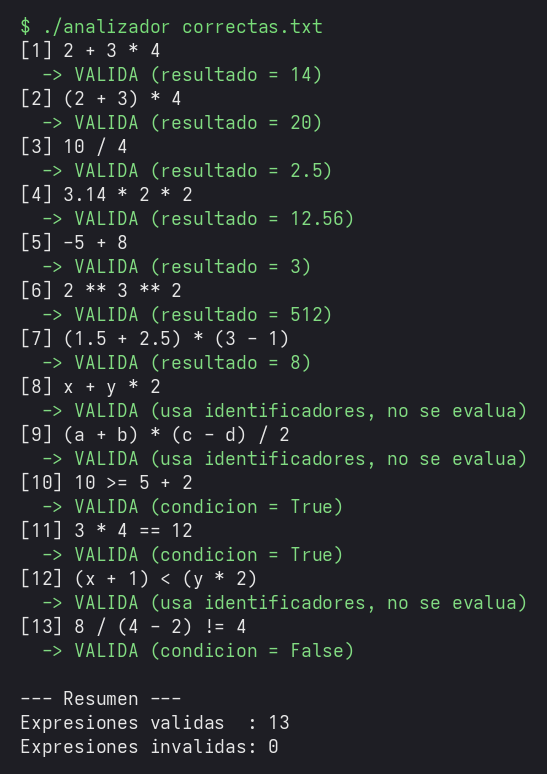
\includegraphics[width=9.5 cm]{imagenes/correctas.png}
    \caption{Salida del analizador sobre correctas.txt.\label{fig:ok}}
    \end{figure}

    \subsection{Archivo con expresiones incorrectas}
    El archivo \texttt{incorrectas.txt} tiene 10 expresiones con errores a propósito:
    \lstinputlisting[numbers=none, caption={Archivo incorrectas.txt.}]{Code/incorrectas.txt}

    En la Figura~\ref{fig:err} se muestra la salida: las 10 se marcaron como inválidas y el analizador no se detuvo en ninguna. En el Cuadro~\ref{tab:errores} se explica la causa de cada una.

    \begin{figure}[H]
    \centering
    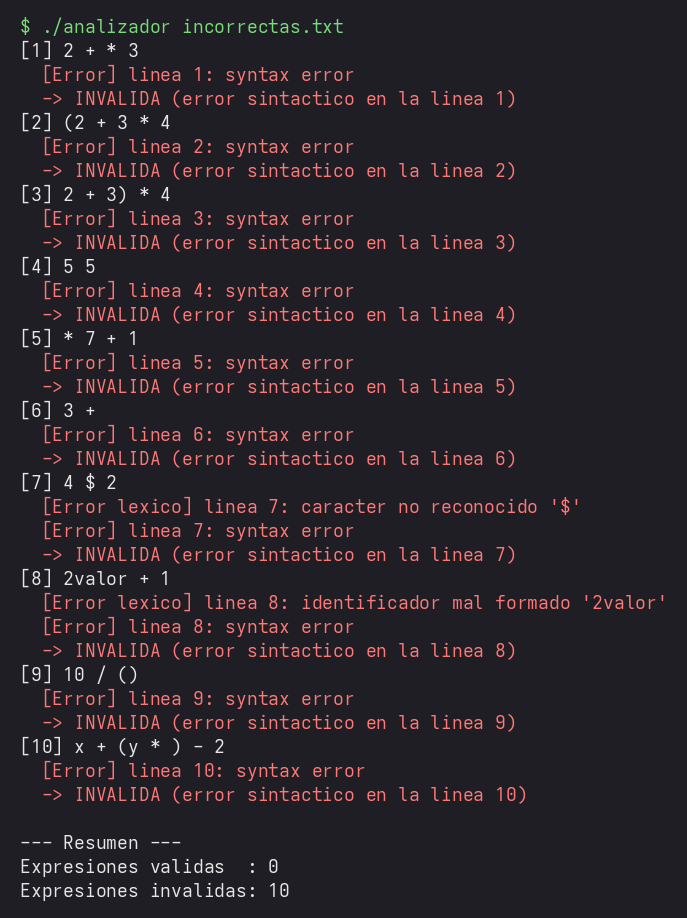
\includegraphics[width=9.5 cm]{imagenes/incorrectas.png}
    \caption{Salida del analizador sobre incorrectas.txt.\label{fig:err}}
    \end{figure}

    \begin{table}[H]
    \begin{center}
    \caption{Errores detectados.}
    \label{tab:errores}
    \begin{tabular}{|c|l|l|l|}
        \hline
        Línea & Expresión & Tipo & Causa \\
        \hline
        1 & \texttt{2 + * 3} & Sintáctico & Dos operadores seguidos \\
        \hline
        2 & \texttt{(2 + 3 * 4} & Sintáctico & Falta cerrar el paréntesis \\
        \hline
        3 & \texttt{2 + 3) * 4} & Sintáctico & Paréntesis de cierre sin abrir \\
        \hline
        4 & \texttt{5 5} & Sintáctico & Dos operandos sin operador \\
        \hline
        5 & \texttt{* 7 + 1} & Sintáctico & Empieza con operador binario \\
        \hline
        6 & \texttt{3 + } & Sintáctico & Falta el segundo operando \\
        \hline
        7 & \texttt{4 \$ 2} & Léxico y sintáctico & Carácter \texttt{\$} no reconocido \\
        \hline
        8 & \texttt{2valor + 1} & Léxico y sintáctico & Identificador mal formado \\
        \hline
        9 & \texttt{10 / ()} & Sintáctico & Paréntesis vacíos \\
        \hline
        10 & \texttt{x + (y * ) - 2} & Sintáctico & Falta un operando dentro del paréntesis \\
        \hline
    \end{tabular}
    \end{center}
    \end{table}

    \subsection{Análisis de los resultados}
    El analizador aceptó todas las expresiones correctas y rechazó todas las incorrectas. Los errores léxicos (líneas 7 y 8) los detectó Lex antes de que Yacc recibiera la cadena, por lo que en esos casos se imprimen dos mensajes: el léxico, que dice cuál es el carácter o lexema problemático, y el sintáctico, porque el token de error que Lex envía no encaja en la gramática. Los errores sintácticos los detectó Yacc en el momento en que llegó un token que ninguna producción permitía en ese punto (por ejemplo, el \texttt{*} de la línea 1 justo después de un \texttt{+}). Gracias a la regla \texttt{error} el análisis se recuperó en cada salto de línea y se reportaron las 10 líneas en una sola pasada.

    Una limitación es que el mensaje de Bison es genérico (\texttt{syntax error}) y no dice qué token se esperaba; se podría mejorar con \texttt{\%define parse.error verbose}. Otra es que las expresiones con variables solo se validan, no se evalúan, porque el programa no tiene tabla de símbolos.
    \newpage

\section{7. Cuestionario}
    \begin{enumerate}
        \item \textbf{¿Qué tipo de errores fueron detectados en los ejemplos incorrectos y cómo influyeron las gramáticas definidas para lograr su identificación?}

        Se detectaron errores léxicos (el carácter \texttt{\$} y el identificador \texttt{2valor}), que no pertenecen a ningún token, y errores sintácticos: operadores seguidos, operandos sin operador, expresiones incompletas y paréntesis desbalanceados o vacíos. Estos últimos se detectan porque la gramática define exactamente en qué orden pueden aparecer los tokens: una \texttt{expresion} solo puede ser un número, un identificador, algo entre paréntesis o dos expresiones unidas por un operador, así que cuando llega un token que no encaja en ninguna producción, Yacc sabe que la cadena no pertenece al lenguaje. En particular, el balance de los paréntesis no se puede comprobar con una expresión regular y se logra gracias a la recursión de la gramática.

        \item \textbf{¿Cómo contribuye el uso de derivaciones por la izquierda o por la derecha en la construcción de un árbol sintáctico para validar las operaciones y las prioridades de las operaciones?}

        La derivación indica en qué orden se expanden los no terminales hasta llegar a la cadena, y cada forma de derivar produce un árbol. Para \texttt{2 * 3 + 4}, si la gramática obliga a que el \texttt{+} se expanda primero (queda en la raíz) y el \texttt{*} después (queda más abajo), el producto se calcula antes que la suma. Por eso la prioridad se logra escribiendo la gramática por niveles, o con \texttt{\%left} y \texttt{\%right} en Yacc. Yacc hace un análisis ascendente que reconstruye una derivación por la derecha, y la asociatividad se refleja en cómo se reduce: con una regla recursiva por la izquierda (\texttt{E -> E - T}) se obtiene \texttt{(8 - 3) - 2}, y con una recursiva por la derecha (\texttt{F -> B ** F}) se obtiene \texttt{2 ** (3 ** 2)}.

        \item \textbf{¿Qué ajustes serían necesarios en la gramática para permitir el reconocimiento de estructuras más complejas, como (a+b)\^{}2, raíz cuadrada, así como operaciones trigonométricas?}

        Para \texttt{(a+b)\^{}2} habría que agregar \texttt{\^{}} como token de potencia (el \texttt{**} ya está) con una regla \texttt{expresion '\^{}' expresion} y mayor prioridad que la multiplicación, asociando por la derecha. Para la raíz cuadrada y las funciones trigonométricas habría que agregar tokens para los nombres (\texttt{sqrt}, \texttt{sin}, \texttt{cos}, \texttt{tan}) en Lex, antes de la regla de identificadores para que no se tomen como variables, y una regla en Yacc del tipo \texttt{expresion: SQRT '(' expresion ')' | SIN '(' expresion ')' | ...}. En una gramática más completa también se podrían agregar funciones con varios argumentos separados por coma, y una tabla de símbolos para guardar las variables.
    \end{enumerate}
    \newpage

\section{8. Conclusiones}
    Con esta práctica entendí cómo se complementan el analizador léxico y el sintáctico: Lex se encarga de los lexemas y Yacc de su orden, y entre los dos se puede validar una expresión completa con muy poco código. Lo que más me costó fue la precedencia y la asociatividad, porque si no se declaran bien los operadores Bison avisa de conflictos y \texttt{2 + 3 * 4} puede dar 20 en lugar de 14; con \texttt{\%left}, \texttt{\%right} y \texttt{\%prec} se resolvió y fue más sencillo que reescribir la gramática por niveles. El WOW fue ver que con la regla \texttt{error '\textbackslash n'} el analizador no se rinde en el primer error y reporta las 10 líneas incorrectas en una sola corrida. El WTF fue un fallo mío: al principio todos los resultados salían como números absurdos (como \texttt{9.88e-324}) porque \texttt{yylval} era un \texttt{int} en el archivo de Lex y un \texttt{double} en el de Yacc; había que definir el mismo \texttt{YYSTYPE} en los dos. También noté que el mensaje por defecto de Bison, \texttt{syntax error}, es poco útil, y que mejoraría con \texttt{parse.error verbose}. En general, la práctica me sirvió para ver cómo un analizador sintáctico de un compilador valida la estructura de lo que escribe el programador.

    \newpage

\section{Referencias Bibliográficas}
    %Formato APA 7° Ed.
    \begin{thebibliography}{100}
        \bibitem{Aho2007}
Aho, A. V., Lam, M. S., Sethi, R., Ullman, J. D. ({\bf 2007}). \emph{Compilers: Principles, Techniques, and Tools}. Segunda edición. Pearson Addison-Wesley. U.S.A.

        \bibitem{Giro2015}
Giró, J., Vázquez, J., Meloni, B., Constable, L. ({\bf 2015}). \emph{Lenguajes formales y teoría de autómatas}. Alfaomega. Argentina.

        \bibitem{Hopcroft2007}
Hopcroft, J. E., Motwani, R., Ullman, J. D. ({\bf 2007}). \emph{Introducción a la teoría de autómatas, lenguajes y computación}. Pearson Educación. México.

        \bibitem{Levine2009}
Levine, J. ({\bf 2009}). \emph{Flex \& Bison}. O'Reilly Media. U.S.A.
    \end{thebibliography}

\end{document}
